\documentclass[12pt, logo=tehranDLDL/ut]{tehranDLDL}
\usepackage{subcaption}
\usepackage{pgfplots}
\usepackage{todonotes}
\usepackage{amsmath}
\usepackage{multicol}

\suptitle{Experiment 5}
\supsubtitle{Sessions 11, 12}
\title{VGA Controller}
\author{Katayoon Basharkhah \& Hadi Safari}
\preparer{Katayoon Basharkhah}
\supervisor{Professor Z. Navabi}
\university{University of Tehran}
\college{College of Engineering\\School of Electrical \& Computer Engineering}
\course[DLLab]{Digital Logic Laboratory}
\coursecode{ECE 045}
\courseurl{https://gitlab.com/hadi_sfr/ut-dldlab/-/jobs/artifacts/master/download?job=build}
\date{Spring 1398}

\graphicspath{{img/5/}}
\pgfplotsset{compat=1.16}

\begin{document}

\maketitle

\tableofcontents
\newpage

\section*{Introduction}
\addcontentsline{toc}{section}{Introduction}

Displaying text is an important function of a video controller. Dedicated circuits are often used to facilitate the display of text characters on a screen. In this experiment, you will learn how to display text or color on a computer-type monitor using the VGA output of DE1 board, as \fref{fig:setup} shows the experiment set-up.

You have to create a character generator circuit for displaying ASCII text characters on the VGA display. The VGA driver in this experiment is capable of displaying characters from a display RAM on a standard VGA monitor. After discussing how a VGA monitor works, we show hardware for driving it. The design methodology presented here uses Verilog blocks, megafunctions, memories and schematic capture. Below is the topics that are explained in the following of this experiment:

\begin{itemize}
    \item VGA driver operation
    \item Monitor synchronization hardware
    \item Character display
    \item VGA driver implementation on DE1 board
\end{itemize}

\begin{figure}[b]
    \centering
    \caption{Experiment set-up\label{fig:setup}}
    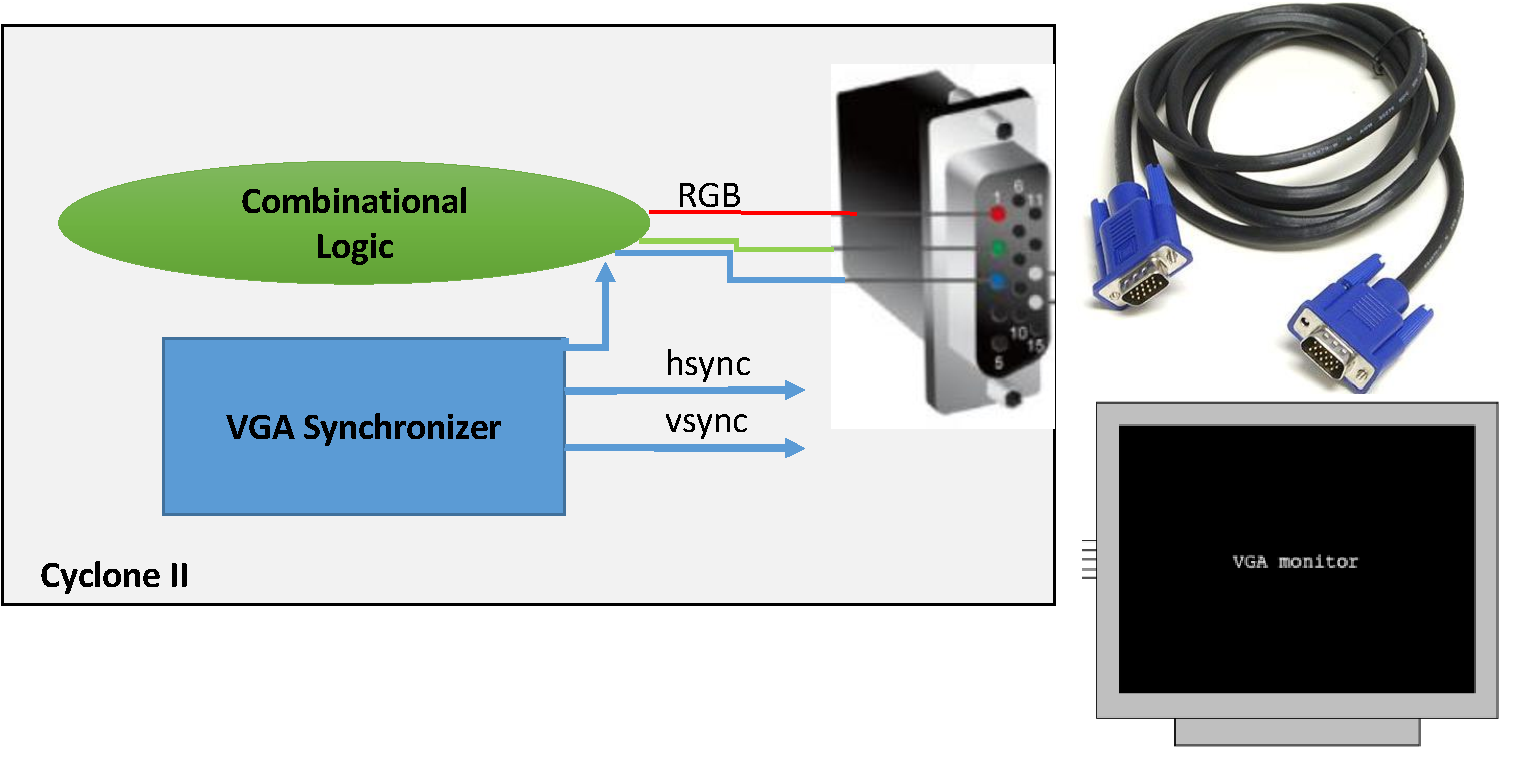
\includegraphics[width=0.6\textwidth]{setup}
\end{figure}

\section{Implementation\label{sec:imp}}

\subsection{VGA Driver Operation}

A standard VGA monitor consists of a grid of pixels that can be divided into rows and columns. A VGA monitor contains at least 480 rows, with 640 pixels per row. Each pixel can display various colors, depending on the state of the red, green and blue input signals. These signals are analog signals and determine the intensity of their corresponding colors. In a VGA monitor pixels are refreshed with proper color one-by-one from location $(0, 0)$ to $(640, 480)$. This is done from upper left corner of the monitor to its lower right corner.

To eliminate any screen flickering, the refreshing must be done such that the entire screen is refreshed, i.e. all screen is swept in less than 0.02 second. For a better than maximum refresh time, of we choose a refresh cycle of $\frac{1}{60}$ of a second. With this rate and considering the overhead time of moving scan from one line to another and one screen to next, a frequency of \SI{25.175}{\mega\hertz} is required for refreshing each pixel.

\subsection{Pixel Sweeping}

For the VGA monitor to work properly, it must receive data at specific times with specific pulses. Horizontal and vertical synchronization pulses must occur at specified times to synchronize the monitor while it is receiving color data.

\begin{figure}
    \centering
    \caption{Pixel sweeping\label{fig:sweeping}}
    \includegraphics[width=0.4\textwidth]{sweeping}
\end{figure}

You can make eight colors on the screen by turning on combinations of the R, G and B. \Fref{tab:rgb} shows the colors you can get with this simple interface.

\begin{table}
\centering
\caption{RGB colors\label{tab:rgb}}
\begin{tabular}{cccr}
Red & Green & Blue & ~\\
\hline
0 & 0 & 0 & Black (\textcolor[rgb]{0,0,0}{$\blacksquare$})\\
0 & 0 & 1 & Blue (\textcolor[rgb]{0,0,1}{$\blacksquare$})\\
0 & 1 & 0 & Green (\textcolor[rgb]{0,1,0}{$\blacksquare$})\\
0 & 1 & 1 & Cyan (\textcolor[rgb]{0,1,1}{$\blacksquare$})\\
1 & 0 & 0 & Red (\textcolor[rgb]{1,0,0}{$\blacksquare$})\\
1 & 0 & 1 & Magenta (\textcolor[rgb]{1,0,1}{$\blacksquare$})\\
1 & 1 & 0 & Yellow (\textcolor[rgb]{1,1,0}{$\blacksquare$})\\
1 & 1 & 1 & White (\textcolor[rgb]{1,1,1}{$\blacksquare$})\\
\end{tabular}
\end{table}

\Fref{fig:refresh-cycle} shows the timing waveform for the color information with respect to the horizontal synchronization and vertical synchronization signal. Times shown are for the standard pixel frequency of 25.175 MHz for 640×480 pixel resolution.

\begin{figure}
    \centering
    \caption{Refresh cycle\label{fig:refresh-cycle}}
    \begin{subfigure}[t]{0.48\textwidth}
        \caption{Vertical\label{fig:vertical-refresh-cycle}}
        \includegraphics[width=\textwidth]{vertical-refresh-cycle}
    \end{subfigure}
    ~
    \begin{subfigure}[t]{0.48\textwidth}
        \caption{Horizontal\label{fig:horizontal-refresh-cycle}}
        \includegraphics[width=\textwidth]{horizontal-refresh-cycle}
    \end{subfigure}
\end{figure}

The hardware required for VGA signal generation must keep track of the number of clock cycles (equivalent pixels) and issue signals according to the timing waveforms of \fref{fig:refresh-cycle}. The Verilog code of code~\ref{lst:synch-verilog} uses the \lstinline{SynchClock} clock signal to generate \lstinline{Hsynch} (\textit{Horizontal Synch} of \fref{fig:horizontal-refresh-cycle}), \lstinline{Vsynch} (\textit{Vertical Synch} of \fref{fig:vertical-refresh-cycle}) and \lstinline{Red}, \lstinline{Green} and \lstinline{Blue} color data.

\begin{lstlisting}[caption={Monitor synchronization hardware\label{lst:synch-verilog}}]
module MonitorSynch (
    input PixelOn, 
    input RedIn, GreenIn, BlueIn, Reset, SynchClock, 
    output Red, Green, Blue, Hsynch, Vsynch,
    output [9:0] PixelRow, PixelCol
);

    reg [9:0] Hcount, Vcount;

    always @(posedge SynchClock) begin
        if (~Reset) Hcount = 0;
        else 
            if (Hcount == 799) Hcount =0; 
            else Hcount <= Hcount + 1;
    end
    always @(posedge SynchClock) begin
        if (~Reset) Vcount = 0;
        else 
            if (Vcount >= 525 && Hcount >= 756) Vcount = 0;
            else if (Hcount == 756) Vcount <= Vcount + 1;
    end

    assign Hsynch = (Hcount >= 661 && Hcount <= 756) ? 0 : 1;
    assign Vsynch = (Vcount >= 491 && Vcount <= 493) ? 0 : 1;
    assign {Red, Green, Blue} = (Hcount <= 640 && Vcount < 480) ? 
        {PixelOn & RedIn, PixelOn & GreenIn, PixelOn & BlueIn} : 0;
    assign PixelCol = (Hcount <= 640) ? Hcount : 0;
    assign PixelRow = (Vcount <= 480) ? Vcount : 0;
endmodule
\end{lstlisting}

The code shown uses color specifications from \lstinline{RedIn}, \lstinline{GreenIn} and \lstinline{BlueIn} input signals and during the time periods specified by parameter $D$ and $R$ in \fref{fig:refresh-cycle}, puts them on the \lstinline{Red}, \lstinline{Green} and \lstinline{Blue} output signals. At any point in time, the Verilog code of code~\ref{lst:synch-verilog} outputs the position of the pixel being updated in its 10-bit \lstinline{PixelRow} and \lstinline{PixelCol} output vectors.

Two \lstinline{always} blocks that are synchronized with \lstinline{SynchClock} keep track of horizontal and vertical counts (\lstinline{Hcount} and \lstinline{Vcount}). \lstinline{Hcount} is associated with parameter $A$ of \Fref{fig:vertical-refresh-cycle} and \lstinline{Vcount} with parameter $O$ of \Fref{fig:horizontal-refresh-cycle}. This Verilog code is defined as a block that will be used in our implementation of a character display design.

\begin{figure}
    \centering
    \caption{Character display hardware\label{fig:char-display}}
    \includegraphics[width=0.7\textwidth]{char-display}
\end{figure}


\subsubsection{Character Display Hardware}

The character pointer hardware is the block shown in upper-right part of \fref{fig:char-display}. \lstinline{MonitorSynch} provides X and Y pixel coordinates for this hardware. \lstinline{CharacterPointer} takes these coordinates and generates a 13-bit address pointing to one of the 4800 characters at the screen location. Because each character consists of 8 rows and 8 columns of pixels, 64 different X and Y coordinates map to the same character address. The Verilog code for generating this mapping is the \lstinline{CharacterPointer} module of code~\ref{lst:character-pointer}.

\begin{lstlisting}[caption={Finding character position from a pixel position\label{lst:character-pointer}}]
module CharacterPointer (input [9:0] PixelRow, PixelCol, output [12:0] CharPntr);
    wire [6:0] ScreenLine, ScreenPos;
    assign ScreenLine = PixelRow [9:3]; // 60 Lines = 480 / 8 (8 is Character Pixel Hight)
    assign ScreenPos = PixelCol [9:3]; // 80 Positions = 640 / 8 (8 is Character Pixel Width)
    assign CharPntr =  ScreenLine * 80 + ScreenPos;
endmodule
\end{lstlisting}

\subsubsection{Pixel Generation Hardware}

The lower part of \fref{fig:char-display} is responsible for generation of a specific pixel value (1 or 0) for the specific X-Y position of screen and the character being displayed. Inputs to this part are ASCII code of the character being displayed (\lstinline{Character[6..0]}) and coordinates within the $\times$ pixel area of the character (\lstinline{PixelRow[2..0]} and \lstinline{PixelCol[2..0]}). The three parts of pixel generation are \lstinline{MatrixSlice}, \lstinline{CharacterMatrix} and \lstinline{CharacterPixel}.

The \lstinline{MatrixSlice} module (Figure 8) takes the ASCII code of the input character and subtracts 32 from it to make printable character codes begin from 0. It then appends three bits of \lstinline{PixelRow} to its right to form an address for the pixel row of the corresponding character.

\begin{lstlisting}[caption={\lstinline{MatrixSlice} Verilog code\label{lst:matrix-slice}}]
module MatrixSlice (input [2:0] PixelRow, input [6:0] Char, output [8:0] MtxPntr);
    assign MtxPntr = {Char - 32, PixelRow[2:0]}; 
endmodule
\end{lstlisting}

The output of this module looks up a row of the character being displayed from the \lstinline{CharacterMatrix} component. In our simple design we use $\times$ character resolution and only support ASCII characters from 32 to 95. With these 64 supported characters, our character matrix becomes an 8-bit memory of 512 words, in which every 8 consecutive words define a character.
For example, as shown in code~\ref{lst:5-cahr-matrix}, pixels for character \texttt{5} with ASCII code of 53 decimal, begin at address \texttt{$\times$A8} hex that is $(53-32)*8$.

\begin{figure}
\begin{lstlisting}[caption={Character matrix for character \texttt{5}\label{lst:5-cahr-matrix}},language={mif},linewidth=0.5\textwidth]
0A8 : 01111110; %   ******
0A9 : 01100000; %   **
0AA : 01111100; %   *****
0AB : 00000110; %       **
0AC : 00000110; %       **
0AD : 01100110; %   **  **
0AE : 00111100; %    ****
0AF : 00000000; %
\end{lstlisting}
\end{figure}

The \lstinline{CharacterMatrix} component is a RAM that is implemented with an Altera~LPM and is mapped into the on-chip memory of our FPGA. This component is called \lstinline{LPM_RAM} and is available under the storage category of Altera megafunctions. Using the megafunction wizard we configure this component as an 8-bit memory with nine address lines. During the configuration process we are asked to enter the Memory Initialization File (\path{.mif}) name, for which we use \path{CharMtx.mif}. Using the \path{mif} format, pixel values (similar to those shown in code~\ref{lst:5-cahr-matrix} for character \texttt{5}) are defined for ASCII characters from 32 to 95. Code~\ref{lst:cahr-matrix} shows the beginning and end of this file, from which its complete format can be seen.

\begin{lstlisting}[caption={Character matrix \texttt{mif} file\label{lst:cahr-matrix}},language={mif}]
DEPTH = 512;
WIDTH = 8;
ADDRESS_RADIX = HEX;
DATA_RADIX = BIN;
% Character Matrix ROM,               %
% addressed by PixelGeneration module %
CONTENT
BEGIN
% ASCII 0010_0000 to 0010_1111  %
000  : 00000000 ; %             %
001  : 00000000 ; %             %
002  : 00000000 ; %             %
003  : 00000000 ; %             %
004  : 00000000 ; %             %
005  : 00000000 ; %             %
006  : 00000000 ; %             %
007  : 00000000 ; %             %
-- ...
1F8  : 00000000 ; %             %
1F9  : 00010000 ; %     *       %
1FA  : 00110000 ; %    **       %
1FB  : 01111111 ; %   *******   %
1FC  : 01111111 ; %   *******   %
1FD  : 00110000 ; %    **       %
1FE  : 00010000 ; %     *       %
1FF  : 00000000 ; %             %
END;
\end{lstlisting}

The output of \lstinline{CharacterMatrix} is \lstinline{q[7..0]}. This output has a slice of the character that is being displayed. For example for row 2 of character \texttt{5}, \lstinline{q[7..0]} is \lstinline[language=mif]{01111100}.

The last component shown in \fref{fig:char-display} that is responsible for pixel generation is \lstinline{CharacterPixel}. This component takes a character row and its column pointer (\lstinline{PixelCol [2:0]}) and looks up the pixel to be displayed. The Verilog code of \lstinline{CharacterPixel} is shown in code~\ref{lst:character-pixel}. This code uses \lstinline{CharColPntr} as index to look into \lstinline{CharacterRow} in reverse bit order.

\begin{lstlisting}[caption={Looking up \lstinline{CharacterPixel}\label{lst:character-pixel}}]
module CharacterPixel (
    input [7:0] CharacterRow, 
    input [2:0] CharColPntr, output Pixel
);
    wire [2:0] index = 
        {CharColPntr[2], CharColPntr[1], CharColPntr[0]};
    wire [7:0] Vector = {
        CharacterRow[0], CharacterRow[1], 
        CharacterRow[2], CharacterRow[3],
        CharacterRow[4], CharacterRow[5],
        CharacterRow[6], CharacterRow[7]
    };
    assign Pixel = Vector [index];
endmodule
\end{lstlisting}

The complete schematic of our character display hardware is shown in \fref{fig:char-display}. The \lstinline{MonitorSynch} module continuously sweeps across the $\times$ pixel screen and refreshes pixel with colors specified by its three color inputs. At the same time it reports the position of the pixel being refreshed to \lstinline{CharacterPointer}. Based on these coordinate, this module calculates the address of the character that is being displayed. After the character is looked up refreshed is found. This pixel value allows color inputs to be used by the \lstinline{MonitorSynch} module for painting the pixel.

The complete design shown in \fref{fig:char-display} is referred to as \lstinline{CharacterDisplay}.

Use the codes provided to you for the character display module and construct the circuit of \fref{fig:char-display} in a block diagram file. 

\designverification{}

\subsection{VGA Driver for Text Data}

The previous section discussed the complete design of \lstinline{CharacterDisplay} hardware. This hardware outputs the address of one of the 4800 characters that is to appear on the screen, looks up its ASCII code, and generates pixel colors and horizontal and vertical synchronization signals.
This section shows a simple VGA driver that provides data to be displayed to our \lstinline{CharacterDisplay} hardware.

The complete schematic of our \lstinline{VGADriver} is shown in \fref{fig:driver}. On the right hand side is \lstinline{CharacterDisplay} that generates character address, monitor synch, and pixel information. On the left hand side is \lstinline{DisplayMemory} that is a dual-port read/write memory. Character address from \lstinline{CharacterDisplay} goes to its read address. The write address, data to be written, and the write enable of this memory are provided externally. While \lstinline{CharacterDisplay} is displaying the current contents of the memory, new data for display can be written into this memory.

\begin{figure}
    \centering
    \caption{VGA driver with display memory\label{fig:driver}}
    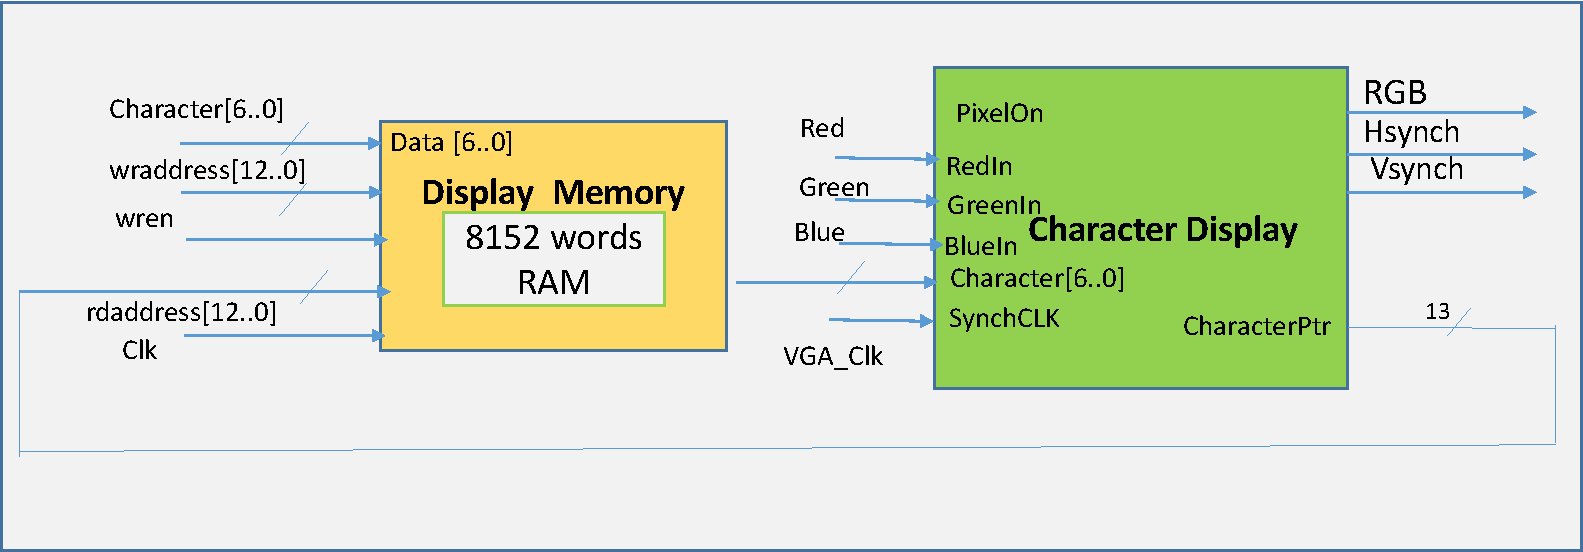
\includegraphics[width=0.7\textwidth]{driver}
\end{figure}

Our \lstinline{VGADriver} has two clock inputs, \lstinline{VGAClk} and \lstinline{MemoryClk}. The latter must be a faster clock so that address output from \lstinline{CharacterDisplay} can be used to lookup the display character from the \lstinline{DisplayMemory}.

Construct the circuit of \fref{fig:driver} in a block diagram file in Quatus~II. Use the block diagrams of the character display design.

\designverification{}

\subsection{VGA Driver Test}

\Fref{fig:tester} shows a simple tester for our VGA driver. This circuit causes the initial data in \lstinline{DisplayMemory} to be displayed on the VGA monitor. Changing display data can only happen by changing contents of \path{DisplayRAM.mif} file which is loaded into this memory.

Note the use of the T-type flip-flop for generating a slower clock for the VGA driver than that of the memory. This circuit is implemented on a UP3 development board and verifies the operation of our VGA adapter. A more elaborate test-bench would have a counter to set memory display memory locations to desired characters. We leave this as an exercise.  

\begin{figure}
    \centering
    \caption{VGA driver tester\label{fig:tester}}
    \includegraphics[width=0.7\textwidth]{tester}
\end{figure}

\begin{itemize}
    \item Construct the circuit of \fref{fig:tester} in a block diagram file. Use the block diagram of the VGA Driver design. Make the proper pin assignment. Although the design has the capability of storing and displaying data from the input ports, you do not have to demonstrate this part. Just show the characters that are stored in the \path{mif} file. So you do not need to assign the character or location ports. Use the \lstinline{SW[2:0]} to change the RGB color and \lstinline{KEY[0]} to reset. For the \lstinline{MemoryClk} use the \SI{50}{\mega\hertz} FPGA Clock. After programming the design on the specified Cyclone device, connect the VGA port to the monitor using the VGA cable available to you.
    \item Test your design and record the results. You should observe some text on the monitor.
\end{itemize}

\designverification{}

\section{Usage}

After understanding the VGA operation and displaying the text on a monitor, now you have to choose one of the task below and complete it. Completing both of these tasks will have an extra point.

\begin{enumerate}
    \item As you have seen in the \nameref{sec:imp} part, the text on the monitor is displayed by $8\times8$ pixel that are small. Change the design to make the text larger but do not change the character pixel size or memory.
    \item Use the Persian alphabet ASCII codes instead of the English ones and write them in \path{mif} file. Then do the same as \nameref{sec:imp} part and show the characters on the monitor.
\end{enumerate}

\designverification{}

\section*{Pre-Lab Assignment}
\addcontentsline{toc}{section}{Pre-Lab Assignment}
Before coming to the lab, answer these questions. The pre-lab needs to be handed in at the start of the lab.

\begin{enumerate}
    \item Explain the MonitorSynch module based on the \fref{fig:refresh-cycle} synchronization timing.
    For more detailed information you can refer to
    ``Embedded Core Design with FPGAs'', McGraw-Hill Electronic Engineering, 2007.
\end{enumerate}


\section*{Acknowledgment}
\addcontentsline{toc}{section}{Acknowledgment}

This lab manual was prepared and developed by \href{mailto:ktbasharkhah@gmail.com?subject=[DLDLab]\%20}{Katayoon Basharkhah}, PHD student of Digital Systems at University of Tehran, under the supervision of professor Zain Navabi.

This manual has been edited by \href{mailto:hadi.safari@ut.ac.ir?subject=[DLDLab]\%20}{Hadi Safari}, undergraduate student of Computer Engineering at University of Tehran.

\end{document}
